\documentclass[12pt, letterpaper]{article}
\usepackage[utf8]{inputenc}
\usepackage{cite}
\usepackage{minted}
\usepackage{url}
\usepackage{graphicx}
\graphicspath{ {./images/} }
\usepackage{csquotes}
\usepackage{hyperref}
\usepackage{tabularx}

\begin{document}

\title{frances: A New AI-web Tool for Analysing NLS Digital Collections}
\author{Wilfrid Askins}
\maketitle

\begin{abstract}
This report describes the design, implementation and evaluation of frances, a web-app developed to make Deep Learning, Natural-Language Processing and Text Mining accessible to an audience of researchers. 

This report builds on existing work in which the prototype of a web tool called frances was created, using AI tools to analyse the Encyclopaedia Britannica. An ontology and knowledge graph were created to describe the relationships between definitions, editions, volumes and more in the encyclopaedia.

This report describes how account functions such as register and login were implemented. The system was split into a front-end and back-end architecture. The system was then containerised to be deployable across various environments.

\end{abstract}

\tableofcontents

\section{Introduction}

\section{Context Survey}

\subsection{Analysis of historical texts}

\subsubsection{Motivation}

\begin{flushleft}
Historical texts are extremely useful for a wide variety of researchers trying to understand history. However, these collections a large amount of content to search through, and require specialist knowledge to understand. This makes historical texts suitable for analysis by Natural Language Processing Technology (NLP) \cite{nlp-historical}. Further work has been done to transform historical collections into graph structures, which creates a database that can be queried using conventional methods. These queries are relatively easy to write and therefore make the text more accessible to non-specialists \cite{rdf-historical}.
\end{flushleft}

\subsubsection{OCR Technology}

OCR (Optical Character Recognition) is technology that translates hand written and printed text into a machine-readable format \cite{ocr-trends}. One typical OCR system used the following stages in-order:

\begin{enumerate}
\item Preprocessing - includes noise removal and enhancement to make the image easier to interpret.
\item Segmentation - involves the segmentation of lines, words and characters, resulting in a set of segmented characters. 
\item Normalisation - segments are resized to remove redundant information from the image.
\item Feature extraction - feature vectors are extracted from the character data.
\item Classification - a neural net is trained to recognise characters from feature vectors.
\end{enumerate}
\cite{ocr-trends}

\subsubsection{NLP Technology}

Natural Language Processing Technology (NLP) is a field in which computers are trained to understand written text in the same way that a human can. NLP divided into two domains, computational and theoretical linguistics. The computational domain is about creating programs which can handle natural language as an input. On the other hand, the theoretical domain is about language universals, i.e. rules which all natural language follows \cite{nlp-fundamentals}. The area of computational linguistics is most relevant to this report, with the follow sub-domains included:

\begin{itemize}
\item Sentance Analysis - determining the meaning of individual sentences.
    \begin{itemize}
    \item Syntax Analysis - determining the structure of sentences, and regularising structure to be consistent between sentences.
    \item Semantic Analysis - finding out what a sentence means, which is determined by finding what conditions make the sentence true.
    \end{itemize}
\item Discourse Analysis - handling the relationships between sentences. These often convey a large amount of implicit information which must be identified before a text can be fully understood.
\end{itemize}
\cite{nlp-fundamentals}

\subsection{Background}

\subsubsection{Information extraction}

Information extraction is the processing of using syntactic, semantic and discourse analysis to identify text features \cite{info-extraction-def}. On example of an Information Extraction System is shown below:

\begin{flushleft}
\begin{figure}[H]
\caption{An example architecture of an Information Extraction System}
\centering
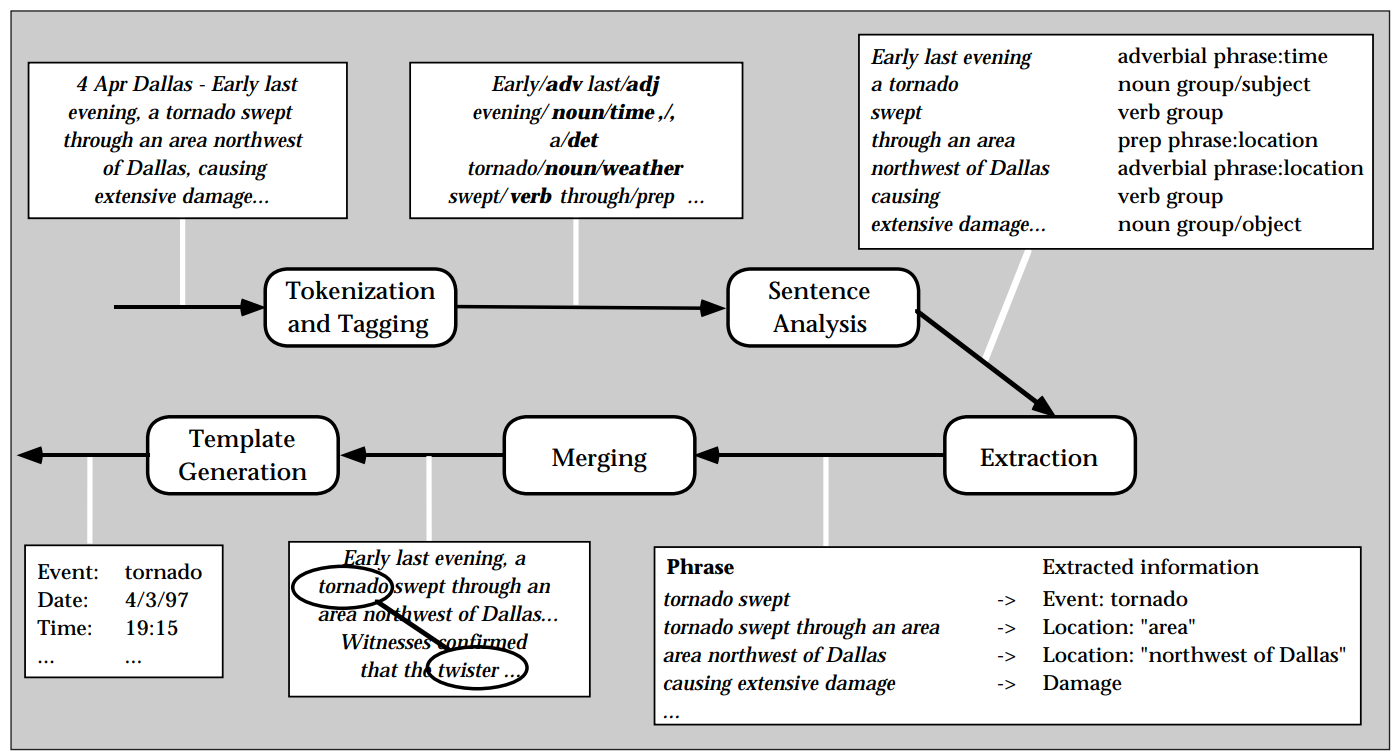
\includegraphics[width=\textwidth]{info-extraction-arch}
\end{figure}
\cite{info-extraction}
\end{flushleft}

One important distinction to understand is that there is a difference between systems that extract text from images, versus systems that extract information from that text. In the example shown above, all three forms of NLP Analysis have been used to create the final result, which contains structured information derived from several sentences of text \cite{info-extraction}.

\subsubsection{Knowledge Graphs}

Knowledge Graphs are data structures which describe the relationships between real world concepts \cite{kg-def}. Each node is a concept (e.g. New York, Michael Jordan) and each edge is a semantic relationship (e.g. lives in, played for) \cite{kg-examples}. A graphical example is shown below:

\begin{flushleft}
\begin{figure}[H]
\caption{An example of a Knowledge Graph}
\centering
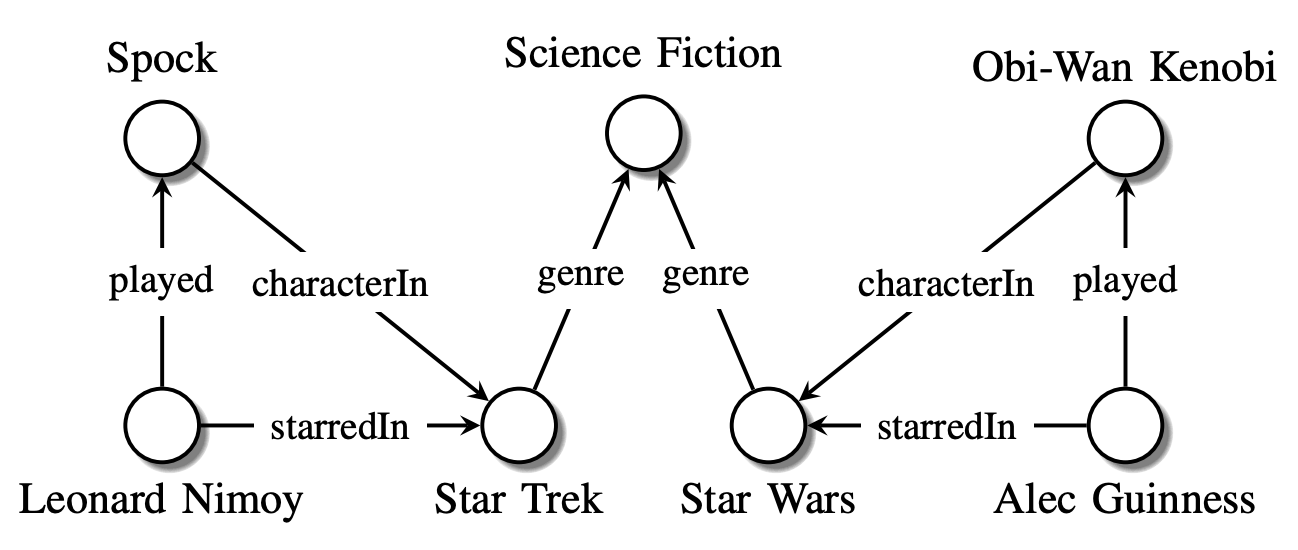
\includegraphics[width=\textwidth]{knowledge-graph-startrek}
\end{figure}
\cite{kg-graphic}
\end{flushleft}

This technology can also be used to predict new features in the world. Machine learning models have been trained on Knowledge Graphs, and have then been used to predict new nodes in the graph. These nodes correspond to new facts about the subject area of the graph \cite{kg-machine-learning}.

\subsubsection{Semantic Web}

\begin{flushleft}
The current world-wide web is designed to be understood by human users
Semantic Web is a plan to create web content that is more machine-readable \cite{semantic-web-primer}.
\end{flushleft}

\begin{flushleft}
It is difficult to understand what the Semantic Web might look like without seeing an example. The following is an extract from a web page that might exist today, advertising a physiotherapist:
\end{flushleft}

\begin{flushleft}
\begin{figure}[H]
\caption{An example web page for a physiotherapist}
\centering
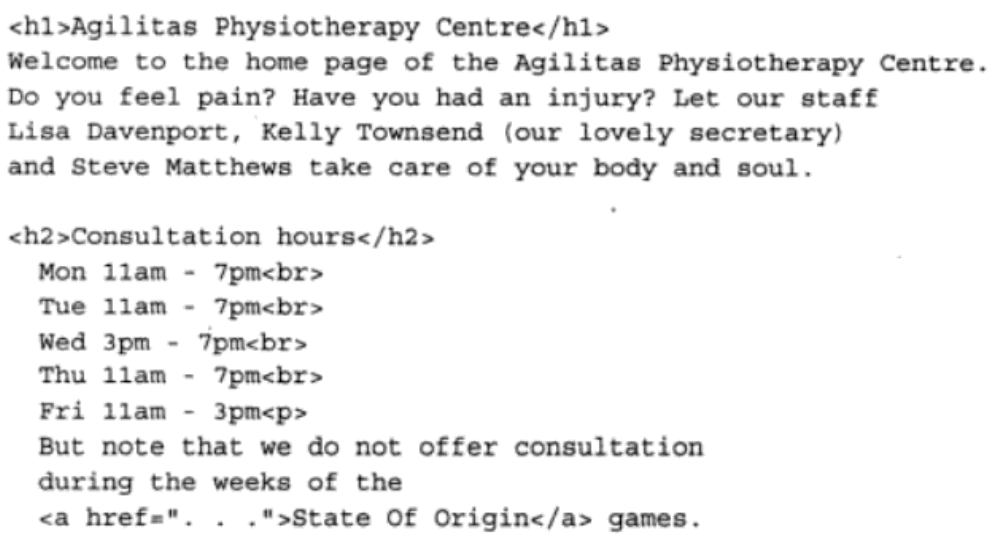
\includegraphics[width=\textwidth]{semantic-before}
\end{figure}
\cite{semantic-web-primer}
\end{flushleft}

\begin{flushleft}
Whereas the following is the Semantic Web equivalent:
\end{flushleft}

\begin{flushleft}
\begin{figure}[H]
\caption{An example of a Semantic Web page}
\centering
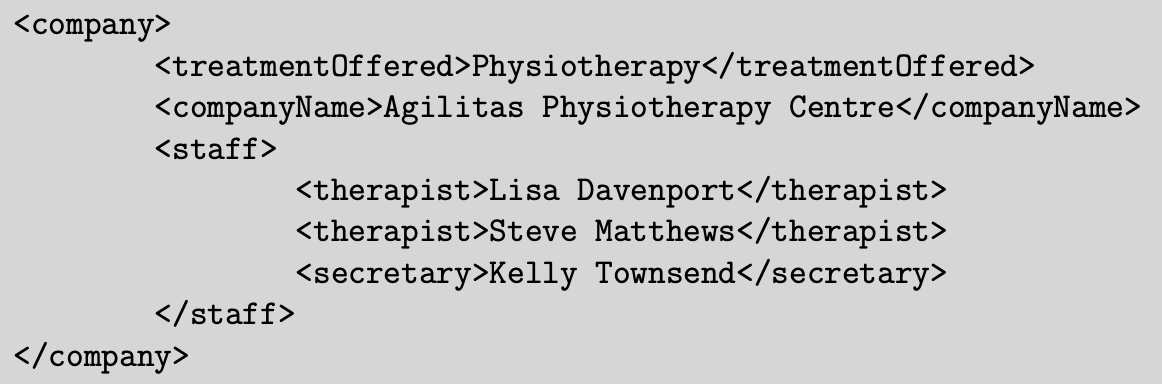
\includegraphics[width=\textwidth]{semantic-after}
\end{figure}
\cite{semantic-web-primer}
\end{flushleft}

The first example is much easier to read for a human, whereas the second is far easier for a machine to read. This form of data would then be combined with a different method of searching, replacing the keyword-based search engines that currently exist \cite{semantic-web-primer}.

\subsection{Relevant Technology}

\subsubsection{Apache Spark}

Apache Spark is a system for executing cluster computing workloads. Spark was originally created to work with RDDs (Resilient Distributed Datasets) which are unique by applying only coarse-grained transformations to data. In other words, a user applies a single operation to each data point. This has the benefit of enabling a high level of parallelism, as computations can be distributed between many machines in a cluster and executed concurrently. Furthermore, it provides fault tolerance by describing a dataset as a result of transformations from a previous dataset. This means an intermediate step or result of a computation can be recreated if lost using the original dataset plus the transformation  \cite{spark-rdds}.

\subsubsection{PySpark}\label{sec:pyspark-desc}

\begin{flushleft}
PySpark is an Apache Spark driver for Python. It enables you to write Spark queries using the provided Python API. It can also create a local Spark master server if needed for development purposes \cite{pyspark-site}.
\end{flushleft}

\begin{flushleft}
Here is an example snippet from the Spark website to better illustrate how PySpark works. It shows a basic Spark session being created, and then the loading and output of a dataframe from a file. A dataframe is essentially an RDD with named columns, in a way that is extremely similar to traditional SQL tables \cite{pyspark-site}.
\end{flushleft}

\begin{minted}{python}
from pyspark.sql import SparkSession

spark = SparkSession.builder.getOrCreate()

# spark is an existing SparkSession
df = spark.read.json("examples/src/main/resources/people.json")
# Displays the content of the DataFrame to stdout
df.show()
# +----+-------+
# | age|   name|
# +----+-------+
# |null|Michael|
# |  30|   Andy|
# |  19| Justin|
# +----+-------+
\end{minted}
\cite{pyspark-dataframes}

\subsubsection{Apache Jena}

Apache Jena is a framework created by the Apache Foundation to create Semantic Web and Linked Data applications. This framework is useful for programs which need to describe both data and relationships between data  \cite{apache-jena}. One commonly used format is RDF (Resource Description Framework) which is a standard to describe graph data \cite{apache-jena}. This data is often exchanged in TTL (Terse RDF Triple Language) files \cite{ttl-files}.

\subsubsection{Apache Jena Fuseki and SPARQL}

Apache Jena Fuseki (usually called Apache Fuseki) is a SPARQL server for the Apache Jena framework. It allows users to upload, store and query RDF files \cite{apache-fuseki}. An example, created by the pre-existing frances project, is shown below:

\begin{minted}{text}
PREFIX eb: <https://w3id.org/eb#>
    PREFIX rdfs: <http://www.w3.org/2000/01/rdf-schema#>
    SELECT ?definition ?term ?year ?enum ?vnum
        WHERE {{
            %s a eb:Article ;
               eb:name ?term ;
               eb:definition ?definition . 
            ?v eb:hasPart %s.
            ?v eb:number ?vnum.
            ?e eb:hasPart ?v.
            ?e eb:publicationYear ?year.
            ?e eb:number ?enum.
            }
            UNION {
            %s a eb:Topic ;
              eb:name ?term ; 
              eb:definition ?definition . 
            ?v eb:hasPart %s.
            ?v eb:number ?vnum.
            ?e eb:hasPart ?v.
            ?e eb:publicationYear ?year.
            ?e eb:number ?enum.
            }
       }  
\end{minted}

\subsubsection{Docker}\label{sec:docker-desc}

\begin{flushleft}
Docker is a platform which containerises applications so they can be deployed operating system agnostically. In order words, apps contained in Docker can run on any machine with the Docker engine installed. This platform is commonly used to deploy microservice architectures to cloud platforms \cite{docker}.
\end{flushleft}

\begin{flushleft}
A Docker image can be created from a base image, with the addition of commands specific to your program. This is defined using a Dockerfile \cite{docker-example}. For example, a basic Flask app (see \hyperref[sec:flask-desc]{Flask Description}) can be containerised with the following Dockerfile:
\end{flushleft}

\begin{minted}{bash}
# The base image
FROM tiangolo/uwsgi-nginx-flask:python3.8-alpine
# Basic system requirement
RUN apk --update add bash nano

# Environment variables for Flask
ENV STATIC_URL /static
ENV STATIC_PATH /var/www/app/static

# Install dependencies
COPY ./requirements.txt /var/www/requirements.txt
RUN pip install -r /var/www/requirements.txt

# Run the Flask server
CMD ["bash", "start.sh"] 
\end{minted}
\cite{docker-example}

\subsubsection{Flask}\label{sec:flask-desc}

Flask is a popular Python web server framework. It provides a number of tools to make development easier including hot reload and template rendering \cite{flask}. Flask makes development extremely quick to begin, with the following shown below being a basic Flask app:

\begin{minted}{python}
from flask import Flask
app = Flask(__name__)

@app.route('/')
def index():
    return '<h1>Hello World!</h1>' 
\end{minted}
\cite{flask}

\subsubsection{Deep Learning Transformers / Hugging Face}

Transformers are the most common form of architecture for Natural Language Processing. This 

Hugging Face is a library that provides a large number of pre-trained models to be applied to a variety of inputs. 

TODO finish

\subsubsection{HashiCorp Consul}\label{sec:consul-desc}
Consul is a service discovery application. In practice, this means that when a service such as a web app launches, it could send a request to Consul to find the IP addresses of its database, caching server and other dependencies. Furthermore it could store configuration information such as the number of threads to run on, or where to log errors to \cite{consul-desc}.

\subsubsection{JSON Web Token (JWT)}\label{sec:jwt-desc}
JSON Web Tokens are a standard of sending information between two communicators \cite{jwt-desc}. They can be used to:

\begin{itemize}
\item Verify the integrity of information. A JWT can be signed so any data changed can be detected and invalidates the token.
\item Hide the payload being sent. A JWT can be encrypted securely using several different secure algorithms, to ensure the privacy of both parties.
\end{itemize}
\cite{jwt-desc}

\subsubsection{OpenAPI}\label{sec:openapi-desc}

OpenAPI is a specification which describes how documents can be written to define APIs (Application Programming Interfaces). Most importantly it includes both a machine-readable description and human-readable info for developers. This means it can be used for both documentation and code generation purposes \cite{openapi}. One relevant part of an OpenAPI document is the paths field, which describes the endpoints that exist for an API. This looks like the following:

\begin{flushleft}
\begin{minted}{yaml}
paths:
  /audio/volume:
    put:
      requestBody:
        required: true
        content:
          application/json:
            schema:
              type: integer
              minimum: 0
              maximum: 11
\end{minted}
\cite{openapi}
\end{flushleft}

The snippet above describes a HTTP PUT endpoint that takes a JSON body. The schema of the body is also defined as containing an integer with set boundaries.

\subsubsection{Swagger}\label{sec:swagger-desc}
Swagger is a set of tools for API Development. This includes Swagger UI, Swagger libraries and many other tools \cite{swagger}.

\paragraph{Swagger UI} is a tool to visualise an OpenAPI Definition (see \hyperref[sec:openapi-desc]{OpenAPI Description}). It will create a local web server which can be navigated to, which will show the following:

\begin{flushleft}
\begin{figure}[H]
\caption{A screenshot of the Swagger UI}
\centering
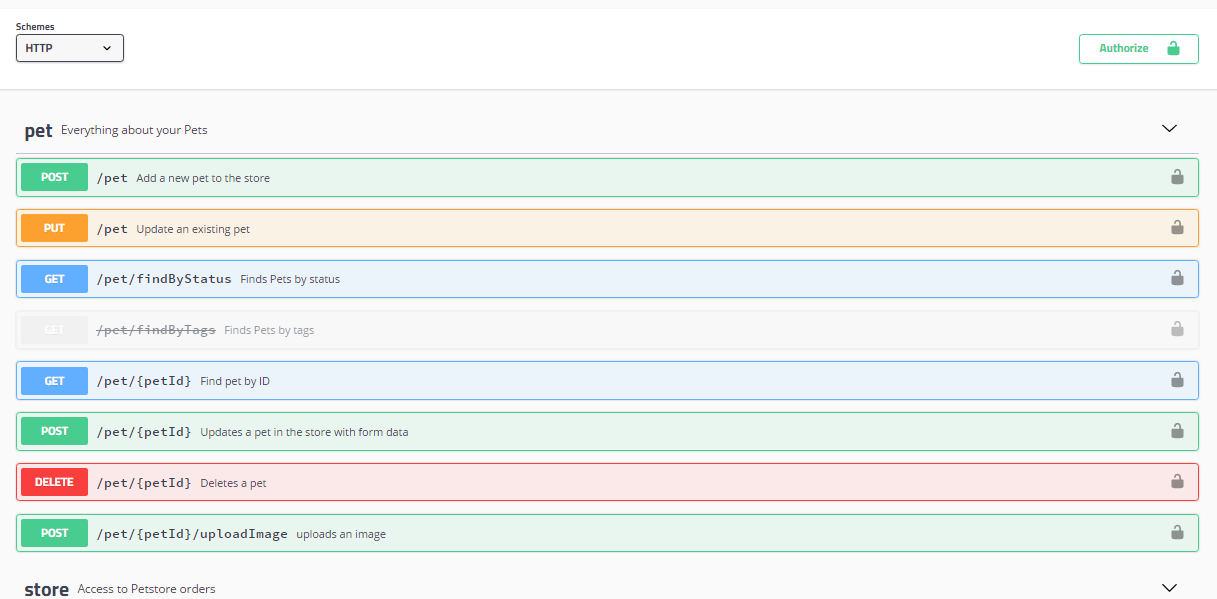
\includegraphics[width=\textwidth]{swagger-ui}
\end{figure}
\cite{swagger-ui}
\end{flushleft}

\begin{flushleft}
This web page will allow a developer to test API requests using the provided forms. This is essentially an auto-generated testing suite in which requests can be generated and sent, and then their responses displayed \cite{swagger-ui}.
\end{flushleft}

\paragraph{Flasgger} is a Python library which integrates Swagger with Flask (see \hyperref[sec:flask-desc]{Flask Description}). It allows quick generation of the Swagger UI using a Flask REST function combined with an OpenAPI specification \cite{flasgger-desc}. This looks like the following:

\begin{minted}{python}
@query.route("/eb_details",  methods=['POST'])
@swag_from("../docs/query/eb_details.yml")
def eb_details():
	...
\end{minted}

The code shown above will automatically generate a Swagger UI from the given file, allowing us to easily test this endpoint.

\subsubsection{React}\label{sec:react-desc}
React is a JavaScript frontend framework created by Facebook to make user interfaces. It uses the concept of components, which are instances describing appearance, behaviour and state \cite{react-desc}. A basic example would look like this:

\begin{flushleft}
\begin{minted}{javascript}
class HelloMessage extends React.Component {
  render() {
    return <div>Hello {this.props.name}</div>;
  }
}

root.render(<HelloMessage name="Taylor"/>);
\end{minted}
\cite{react-desc}
\end{flushleft}

\begin{flushleft}
This component will render a basic "Hello Taylor" message to the user. Components can become more complicated by handling state changes, e.g. from mouse clicks. This makes React an incredibly powerful way of creating a complex and interactive user interface \cite{react-desc}.
\end{flushleft}

\subsubsection{Universally Unique Identifiers (UUIDs)}\label{sec:uuids-desc}

TODO write

\subsection{Pre-existing work}

\subsubsection{NLS Digital Collections}

The National Library of Scotland (NLS) provides many digital collections, which are historical collections in the same sense that a museum might offer. A large part of these collections come from the mass digitisation program of books, maps, manuscripts and newspapers. However, they also include more than 5 million e-books and e-journals \cite{nls-collections}.

\begin{flushleft}
The NLS has over 5PB stored in the library as of 2020. The NLS Data Foundry makes a large portion of this open to the public, available to download in several formats:
\begin{itemize}
\item METS - a format describing digital objects.
\item ALTO - used to store layout information.
\item OCR - text and image files resulting from Optical Character Recognition.
\end{itemize}
\cite{nls-collections}
\end{flushleft}

\subsubsection{Defoe analysis library}

\begin{flushleft}
Defoe is a Python library that provides tools to analyse historical texts using Apache Spark. It provides a number of pre-made queries, with their results being computed in parallel \cite{defoe}. 
\end{flushleft}

\begin{flushleft}
The library's queries take parameters allowing a user to customise them. For example, the query "uris\_keysearch" will find the URIs (Universal Resource Identifier) of terms with the given keywords, returning them grouped by year \cite{defoe}.
\end{flushleft}

\begin{flushleft}
Defoe is primarily designed to make digital collections more accessible to academics working in the humanities. These researchers would previously have had little access to HPC (High Performance Computing) but can use defoe on the command-line in many different environments (personal laptops, cloud platforms, etc) \cite{defoe}.
\end{flushleft}

\subsubsection{EB Ontology and EB Knowledge Graph}

An ontology as described in this report is a formal specification of a model of concepts and their relationships \cite{ontology}. EB Ontology is an ontology describing the relationships between definitions, editions, volumes and more in the Encyclopaedia Britannica \cite{eb-ontology}. The following is a diagram of these links:

\begin{flushleft}
\begin{figure}[H]
\caption{A diagram of the EB Ontology}
\centering
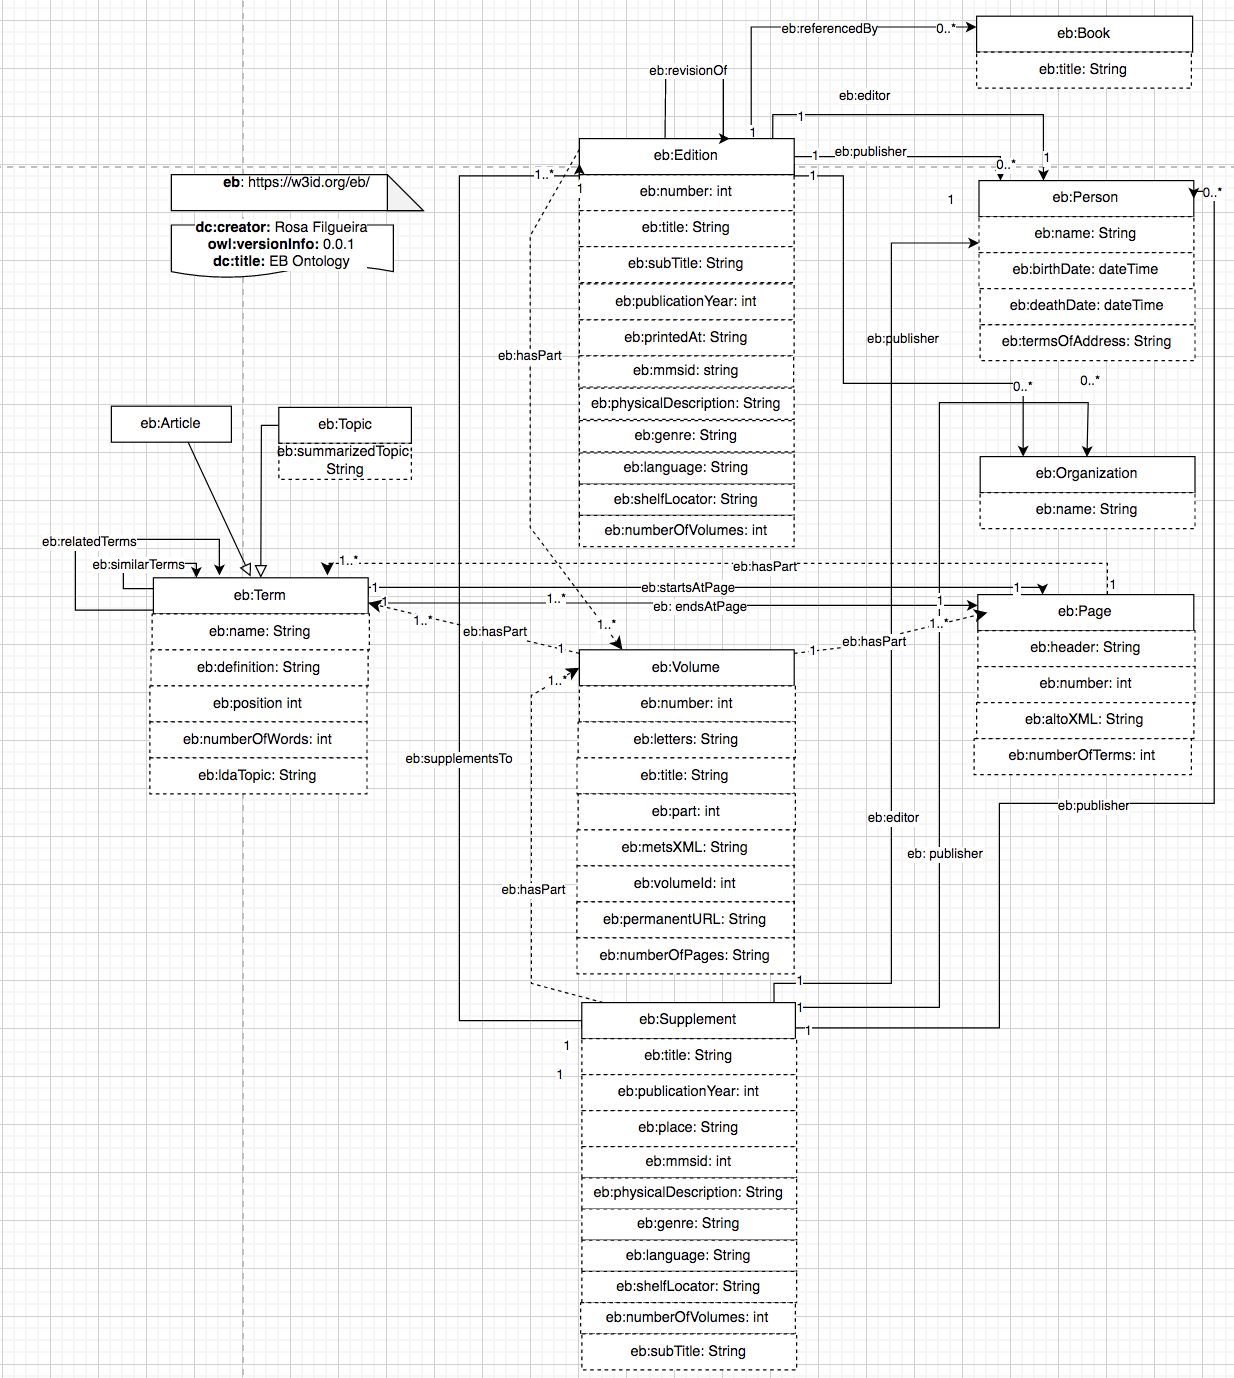
\includegraphics[width=\textwidth]{eb-ontology}
\end{figure}
\cite{eb-ontology}
\end{flushleft}

With this in mind, EB Knowledge Graph (also referred to as EB-KG) is then the knowledge graph created using EB Ontology and the data extracted from the Encyclopaedia Britannica. The distinction is that EB Ontology refers to the abstract relationship between entities in the encyclopaedia, whereas EB-KG is a collection of instances of these entities and relationships \cite{eb-ontology}.

\subsubsection{Frances web app}

\begin{flushleft}
Frances is a web app, which the prototype of was created prior to this report. Frances allows users to query the EB Knowledge Graph to gain insights about the Encyclopaedia Britannica. For example, a user could search for a term and see it's usages. The term could then be spell checked to remove mistakes from the definition. Finally, the term could be visualised to see how often it is used in the encyclopaedia.
\end{flushleft}

\begin{flushleft}
Frances also allows users to execute defoe queries using the web interface. This is more accessible than the command-line interface defoe previously offered. 
\end{flushleft}

\section{Requirements}
\subsection{Functional}

The following requirements are about the how the system should function. They are derived from a combination of the following sources:

\begin{flushleft}
\begin{itemize}
\item The old version of frances. The code and functionality of this app was examined and used to determine its original requirements.
\item The new functionality that this project aims to implement, as discussed with my supervisor Rosa Filgueira.
\end{itemize}
\end{flushleft}

\renewcommand{\arraystretch}{1.5}

\begin{center}
\begin{tabularx}{\textwidth}{ c X c }
 ID & Description & Dependencies \\ 
 \hline
  UF1 & The system shall search a term in EB, and get the search results with their definitions, term type, uri for information visualisation, related terms, metadata information (year, edition, volume, start page, end page), and advanced analyses results (topic modelling, sentiment score, term similarity, spelling checking and summarisation). &  \\ 
 UF2 & The system shall check original images from NLS of the start page or end page of the term search result. & UF1 \\ 
 UF3 & The system shall get term information of related terms from previous term search result. & UF1 \\ 
 UF4 & The system shall generate a visualisation of each topic mode found in term search results. For each topic model, plot their most common 10 words, along with their c-TF-IDF scores. & UF1 \\ 
 UF5 & The system shall generate a visualisation of how similar each topic mode found in term search results is to each other. & UF1 \\ 
 UF6 & The system shall require the user to create an account with username, password and email to gain access to defoe queries. &  \\ 
 UF7 & The system shall ask the user to login or register an account if the user tries to use the defoe queries function without logging in. &  \\ 
 UF8 & The system shall deny user access to other functions except defoe queries related without login. &  \\ 
 UF9 & The system shall only use EB collection when it comes to Term search, similarity, topic modelling and spell checker. & \\
 UF10 & The system shall support EB, Chapbook and Gazetteers collections for both defoe queries and collection details functions. & \\
\end{tabularx}
\end{center}

\subsection{Non-Functional}

\begin{center}
\begin{tabularx}{\textwidth}{ c X }
 Name & Description \\ 
 \hline
 Availablity & Measured by 99.99\% across 1 hour of typical traffic. \\ 
 Portability & Across Windows, MacOS and Linux operating systems without any code changes. \\ 
 Reliability & Measured by a MTTF (Mean time to failure) of 10,000 hours.   \\ 
 Performance & Measured by fulfilling 99.9\% of standard requests in under 200ms over 1 hour of typical traffic. \\ 
 Scalability & Measured by supporting the execution of 3 or more defoe queries at once. \\ 
\end{tabularx}
\end{center}

\section{Software Engineering Process}

\subsection{Methodology}
\subsubsection{Agile Methodological Approach}

The Agile manifesto describes the Agile methodology, which is summarised as:

\begin{displayquote}
    \begin{itemize}
    \item Individuals and interactions over processes and tools
    \item Working software over comprehensive documentation
    \item Customer collaboration over contract negotiation
    \item Responding to change over following a plan
    \end{itemize}
    \cite{agile-manifesto}
\end{displayquote}

\begin{flushleft}
These are the principles we decided to follow during this project. These make sense to follow because they are more suitable for smaller teams and projects, in comparison to more structured approaches such as the Waterfall method \cite{waterfall}. Furthermore, the relatively open requirements and short timescale for this project meant that significant adjustments would be made depending on the progress made on the final product.
\end{flushleft}

\begin{flushleft}
However, it should be noted that traditionally in industry, the Agile principles would be implemented using a framework such as Scrum, which describes how a team should function in an Agile manner \cite{scrum}. The process is explained below: 

\begin{figure}[H]
\caption{Scrum framework diagram}
\centering
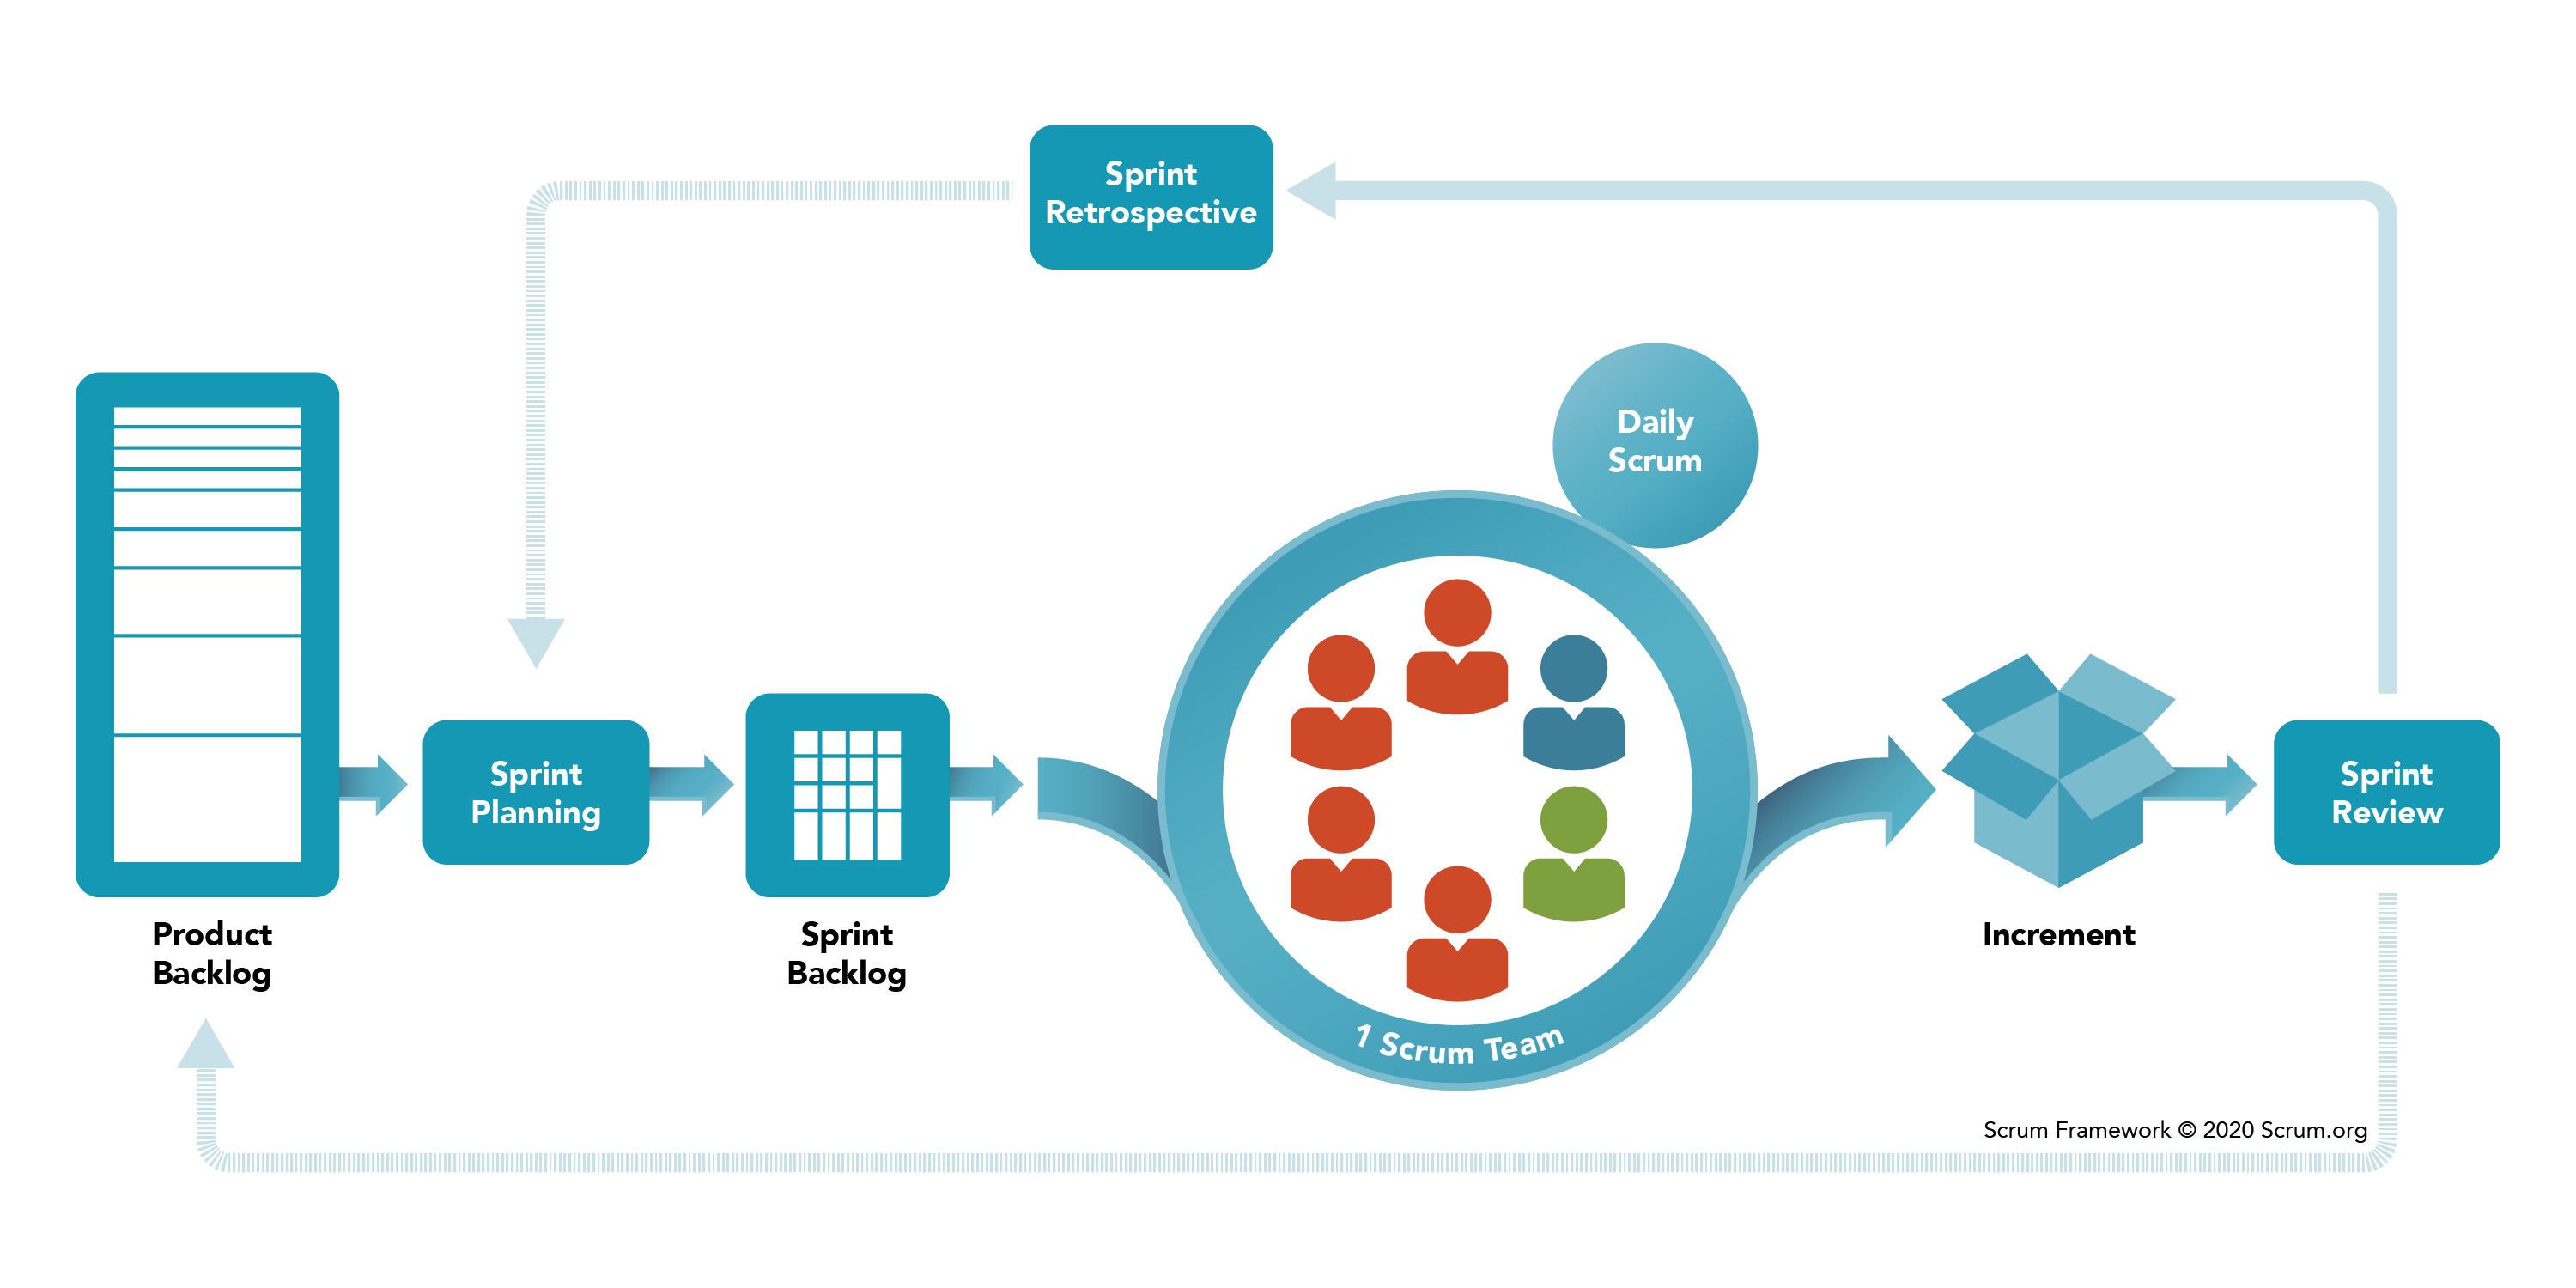
\includegraphics[width=\textwidth]{scrum}
\end{figure}
\cite{scrum}
\end{flushleft}

While Scrum can be beneficial to small teams and projects, our team only consisted of two members with one primary stakeholder (our supervisor). For this reason, a formal process with a sprint planning, backlog and retrospective didn't make sense. This is why throughout the project the team operated informally. We would meet once per week to discuss what we had worked on, which is reminiscent of the transparency principle from the Scrum methodology \cite{scrum}. However, we only verbally communicated our sprint planning and retrospective. Furthermore, our backlog was simply the remaining project requirements, as the work included in our project had a well defined limit. 

\subsubsection{Test-driven implementation}

Test-driven development (TDD) was followed relatively closely in the development of this project, with a few exceptions. We chose to follow this methodology because it is believed to produce more reliable software than untested methods. A basic explanation of TDD is as follows:

\begin{itemize}
\item A test is created based off of a project requirement.
\item When first run, the test fails as the project doesn't currently fulfil it.
\item The minimum amount of code is written to make the test pass.
\item The code is refactored for readability and maintainability.
\item This process is repeated for the full development of the project or submodule.
\end{itemize}
\cite{test-driven-dev}

It should be mentioned that this was process adapted significantly for this project, as we weren't dealing with a greenfield project \cite{greenfield-project}. Because we had pre-existing code to adapt, we obviously couldn't create tests before the code, as the code already exists. For this reason, it was decided that Swagger should be used to retroactively create tests for the frances API (see \hyperref[sec:swagger-desc]{Swagger Description}. This tool was used to write documentation for HTTP APIs, then automatically create a HTTP client with default request values. This could then be used to test the API \cite{swagger}. This was a compromise due to the small timeframe. Had we had longer, end-to-end and unit tests could have been created for all areas of the project. Swagger is a good alternative because it provides both documentation and testing in a smaller development time \cite{swagger}.

\subsection{Task Allocation}

Task allocation in this project was handled informally and on an ad-hoc basis depending on individual requirements. However, the tasks allocated can be divided fairly cleanly into the following groups (with some small exceptions):

\setlength{\arrayrulewidth}{0.5mm}
\setlength{\tabcolsep}{18pt}
\renewcommand{\arraystretch}{1.5}

\begin{center}
\begin{tabular}{|p{0.5\textwidth}|p{0.5\textwidth}|} 
 \hline
 Task name & Members Assigned \\ [0.5ex] 
 \hline
  Frontend interface & Damon Yu \\
  Backend authentication & Damon Yu \\
  Backend API & Wilfrid Askins \\
  Database queries & Damon Yu, Wilfrid Askins \\
  Defoe library & Wilfrid Askins \\
  Deployment & Wilfrid Askins \\
 \hline
\end{tabular}
\end{center}

\section{Ethics}
This project was relatively low-risk ethically for a number of reasons:
\begin{itemize}
\item The project analyses data that is publicly available, meaning that most of the project has zero privacy risk.
\item The scope of our report is only on software development, and doesn't require us to conduct any research on real subjects (e.g. interviewing people and collecting data).  
\end{itemize}

However, the project did have some small areas which had to be focused on:

\begin{itemize}
\item The project holds user account data which could contain sensitive data (full names, passwords, etc).
\item The project exposes a web server which could compromise user's machines to malicious actors.
\end{itemize}

\begin{flushleft}
    Overall, these ethical factors had to be considered in the design and implementation of the application. The following should be done to ensure this:
    
    \begin{itemize}
    \item Database security features
        \begin{itemize}
        \item All database configuration should be done dynamically with options for any IP address, username and password. This means that account data can be held in a PostgreSQL database configured securely and separately from the main application. The alternative is hardcoded values in the same way as frances was previously configured, but this is inherently risky from a security perspective.
        \item If possible, all database connections should stay within the container orchestration network, meaning no outside connection from bad actors is possible.
        \item Account passwords should always be hashed, meaning a data leak will not expose the real values of user passwords.
        \end{itemize}
    \item Web server security features
        \begin{itemize}
        \item Users shouldn't be able to input file paths outside the application's root directory, as this could be used to access a host machine remotely.
        \item When running defoe, users shouldn't be able to execute arbitrary shell commands, as this could be used for a wide variety of malicious goals.
        \end{itemize}
    \end{itemize}
\end{flushleft}

\section{Design}

\subsection{System Architecture}

The system architecture was designed using the Component diagram from the C4 Model. This is a viewpoint set which describes what diagrams should be included in the documentation of an architecture \cite{c4-model}. However, since we are updating an existing system, the only diagram that is required is the Component diagram. This is because the other viewpoints (System Context, Container, Code) have already been decided by pre-existing work so won't be changed throughout this report.

\begin{figure}[H]
\caption{The System Architecture at the component level}
\centering
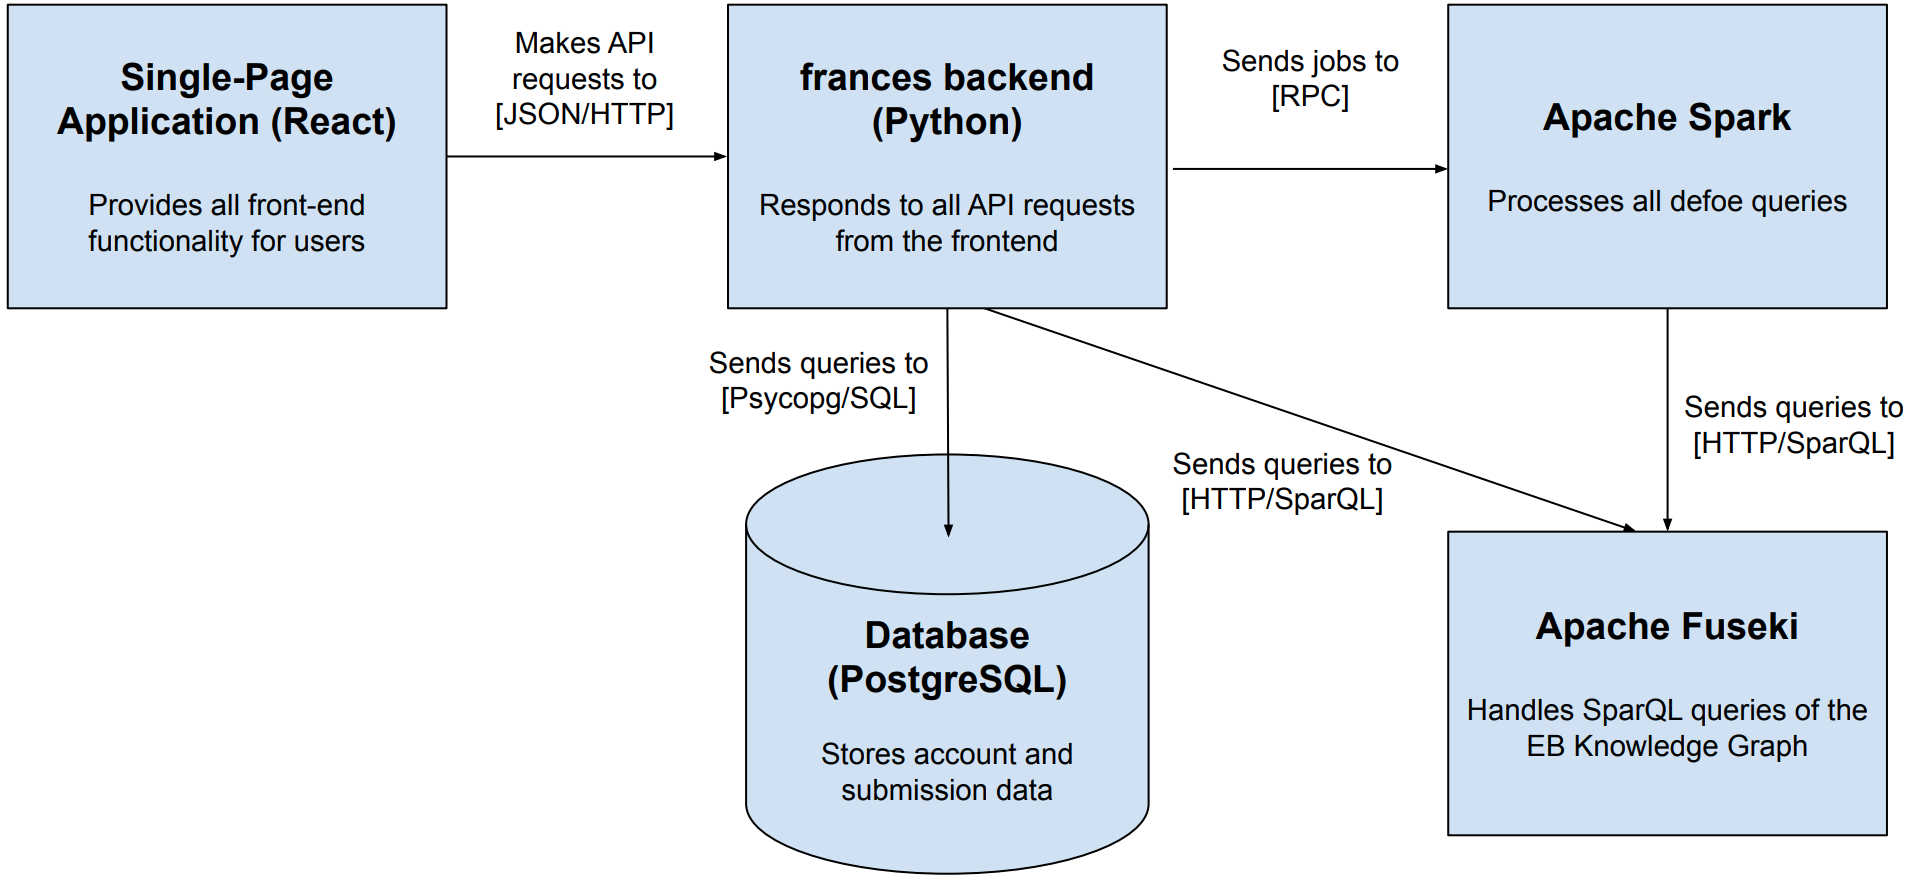
\includegraphics[width=\textwidth]{arch-components}
\end{figure}

\subsection{Frontend}

The application's frontend was previously HTML returned from the pre-existing Flask app. However, since the architecture split the system into frontend and backend, this made it a difficult choice to decide which framework was suitable for the frontend.

\subsection{Storage Solutions}
\subsubsection{ElasticSearch}
\subsubsection{PostgreSQL}

\begin{flushleft}
PostgreSQL was selected as the database software for this project over MySQL. The two DBMS (Database Management Systems) are extremely similar but PostgresSQL offers slightly better features for customisation of constraints, data security and recovery \cite{postgres}. While these aren't enormously important pressures on the project, this made it the preferred solution.
 \end{flushleft}

\begin{flushleft}
Note that this app was designed to use PostgreSQL directly, instead of an ORM (Object-relational Mapper) library such as SQLAlchemy \cite{sql-alchemy}. This was a difficult choice to make because each option has some major advantages. On the one hand, SQLAlchemy would have reduced the development time significantly by requiring no code to read and write to the database. However, it also presented the risk that the ORM would lack some functionality we'd want from our system. For this reason, it was the safer but slightly slower choice (in terms of development speed) to use PostgreSQL directly over SQLAlchemy.
 \end{flushleft}

\subsection{Deployment}
\subsubsection{Containerisation}

To containerise the application, the choice was made to use Docker, which is a framework to package a program in a container which emulates an operating system (see \hyperref[sec:docker-desc]{Docker Description}). Docker was a good choice for this technology because it is free and open-source \cite{docker}. Furthermore, it is very popular in the industry, being used by 50\% of deployments \cite{docker-stats} and therefore will be easier to maintain in the future by other contributors.

\subsubsection{Local environment}

To deploy the project to a local environment, the tool Docker Compose was chosen. This was a natural choice because it comes packaged with the default Docker installation. By creating a YAML config file, a user can describe a number of containers with a network between them. This config file can then be run locally by a user to create the app and its dependencies \cite{docker}.

\subsubsection{Cloud platform}

When deployed to a cloud platform, the choice was made to use the tool Terraform. This software is an IaC (Infrastructure as Code) tool which uses config files to create a deployment in the cloud. This has the benefit of being able to both deploy the project, and describe the deployment to future researchers. Furthermore, the deployment can be reproduced consistently by anyone using the Terraform command-line app \cite{terraform}.

\section{Implementation}

\subsection{Frontend}\label{sec:frontend}

\subsection{Database}

\subsubsection{Abstraction of operations}\label{sec:absraction-of-operations}

If we had queries written everywhere in the API endpoints, it would be extremely difficult to understand, debug and test. To solve this problem, database operations were handled by the Database class (see Appendix \ref{appendix:db.py}). An extract from this class shows some of the typical functions:

\begin{minted}[breaklines]{python}
    def get_user_by_email(self, email):
        sql = "SELECT userId,firstName, lastName,email,password FROM Users WHERE Email=%s;"
        cursor = self.db.cursor()
        cursor.execute(sql, (email,))

        results = cursor.fetchall()
        if len(results) == 0:
            return None

        res = results[0]
        return User(*res)

    def add_user(self, user):
        sql = "INSERT INTO Users (userId, firstName, lastName, email, password) VALUES (%s, %s, %s, %s, %s);"
        vals = (user.id, user.first_name, user.last_name, user.email, user.password)

        cursor = self.db.cursor()
        cursor.execute(sql, vals)
        self.db.commit()
        return
\end{minted}

These functions all work with the same data classes. This means that a user returned by one function can be consumed by another. The user class looks like the following:

\begin{minted}[breaklines]{python}
class User:
    def __init__(self, id, first_name, last_name, email, password):
        self.id = id
        self.first_name = first_name
        self.last_name = last_name
        self.email = email
        self.password = password

    @staticmethod
    def create_new(first_name, last_name, email, password):
        id = uuid.uuid5(uuid.NAMESPACE_URL, namespace + first_name + str(time.time()))
        return User(id, first_name, last_name, email, password)
\end{minted}

Note that all IDs in the database are UUIDs (see \hyperref[sec:uuids-desc]{UUIDs Description}) created in Python code, rather than an integer auto-incremented by the database. This choice was made because of several factors:
\begin{itemize}
\item UUIDs are more secure than sequential integer IDs, as they do not given users information about the range of records stored \cite{uuids-compare}.
\item Both PostgreSQL and Python's PostgreSQL bindings support UUIDs. However, they don't support returning a UUID from a record insertion \cite{uuids-support}.
\item UUIDs created in Python can in theory cause errors if two are generated the same by random chance, but this is extremely unlikely to happen \cite{uuids-what-is}.
\end{itemize}

\subsubsection{Table creation on startup}

Every time the frances web server starts up, it connects to the database. The first operation it runs is shown below, which is to read the tables creation file and execute it.

\begin{minted}{python}
    def create_tables(self):
        f = open(tables_file_path, "r")
        queries = f.read()
        self.db.cursor().execute(queries)
        self.db.commit()
\end{minted}

This file contains a collection of SQL statements which describe the entire table structure (see Appendix \ref{appendix:tables-sql}). They are all defined so that the app can be connected to an empty database, and still work immediately by creating all required tables. This is extremely useful because database deployment will be successful in any environment, so long as the database connection details are correct.

\subsection{Backend}

\subsubsection{API creation}

\begin{flushleft}
The pre-existing code didn't expose an API publicly, instead it used endpoints which returned rendered HTML templates. This essentially means that the frontend and backend are merged together. While this approach is fine for small and simple applications, it becomes an increasing problem when apps become large and complex. To fix this from the backend perspective, the frances web server had to be updated to return a backend API response rather than a rendered page. The old version looked like this:
\end{flushleft}

\begin{minted}[breaklines]{python}
    return render_template("results.html", results=results_for_render,
                                           pagination = pagination, 
                                           headers=headers,
                                           term=term, bar_plot=bar_plot, heatmap_plot=heatmap_plot)
\end{minted}

\begin{flushleft}
Because React (see \hyperref[sec:react-desc]{React Description}) was chosen as a frontend framework (see \ref{sec:frontend}), it made sense to work with data that React could handle effectively. Traditional HTTP APIs often use form data, in which the data is defined directly in the HTML, with the request built by the browser and sent to defined endpoint \cite{html-forms}. This is different to how React apps often handle data. Because React is a JavaScript framework, it often works with responses in JSON (JavaScript Object Notation). This is incredibly easy to use because the language supports it by default \cite{react-json}. Furthermore requests can easily be asynchronous if needed, in comparison to HTML forms which are inherently not \cite{html-forms}. This decision changed the previous code to this:
\end{flushleft}

\begin{minted}[breaklines]{python}
    return jsonify({
        "results": results_for_render,
        "pagination": pagination_to_dict(pagination),
        "headers": headers,
        "term": term,
        "bar_plot": figure_to_dict(bar_plot),
        "heatmap_plot": figure_to_dict(heatmap_plot),
    }), HTTPStatus.OK
\end{minted}

\subsubsection{API documentation and testing}

\begin{flushleft}
Since this project involved creating an API, it was important to document and test it in order to make it reliable and maintainable. The only issue was that we had an extremely limited amount of time to work on this, so we needed to finish it efficiently. The solution was to use Swagger and Flasgger (see \hyperref[sec:swagger-desc]{Swagger Description}) to write a basic OpenAPI document for each endpoint (see \hyperref[sec:openapi-desc]{OpenAPI Description}) and then autogenerate the Swagger UI test suite. The following shows the document for the volume details endpoint:
\end{flushleft}

\begin{minted}{yaml}
Volume Details
---
tags:
  - Query
consumes:
  - application/json
parameters:
  - in: body
    name: payload
    schema:
      type: object
      properties:
        edition_selection:
          type: string
          description: The edition to list the volumes of.
responses:
  201:
    description: Volumes list
  400:
    description: Invalid input
\end{minted}

\subsubsection{Enabling user accounts}

Creating a user account system was one of the more complex parts of the system's implementation. It involved several steps:
\begin{itemize}
\item Creation of the account records stored in the database (see \hyperref[sec:absraction-of-operations]{Abstraction of operations}).
\item Authorising and protecting specific routes.
\item Issuing tokens to authorise accounts.
\item Account security features.
\end{itemize}

\paragraph{Account security features}

accounts have UUIDs (see \hyperref[sec:uuids-desc]{UUIDs Description}) which has been discussed in depth previously (see \hyperref[sec:absraction-of-operations]{Abstraction of operations})
accounts have passwords hashed
example of password hashing code

\paragraph{Issuing access and refresh}

\begin{flushleft}
Our implementation of authentication uses an OAuth 2.0 scheme to issue access and refresh tokens. In this scheme, access tokens are used to authenticate a user when calling an API. Refresh tokens are then used to get new access tokens \cite{oauth-2}. My partner used JWT as the format for these tokens (see \hyperref[sec:jwt-desc]{JWT Description}) because they are a standard format with strong security features built in.
\end{flushleft}

\begin{flushleft}
When a user logs in, an access and refresh token are created based on that user's ID. These tokens are set as HTTP Cookies, which are items of data with a limited size that are stored in the end user's web browser. They can then be used by the server to identify that browser again in future requests, making them useful for handling login data such as this \cite{http-cookies}. As the user attempts to log in, their password is checked, then the cookies are set as shown below.
\end{flushleft}

\begin{minted}{python}
            access_token = create_access_token(identity=user.id)
            refresh_token = create_refresh_token(identity=user.id)
            ...
            set_access_cookies(response, access_token)
            set_refresh_cookies(response, refresh_token)
\end{minted}

\begin{flushleft}
This access token can then be refreshed using the token refresh endpoint as shown below.
\end{flushleft}

\begin{minted}{python}
@auth.post("/auth/token/refresh")
@jwt_required(refresh=True)
@swag_from("../docs/auth/refresh.yml")
def refresh_token():
    user_id = get_jwt_identity()
    access_token = create_access_token(identity=user_id)
    response = jsonify({
        "refresh": True
    })
    set_access_cookies(response, access_token)
    return response, HTTPStatus.OK
\end{minted}

\paragraph{Protected routes}

\begin{flushleft}
Finally, the following shows how this authentication scheme works on protected routes. These routes must have the jwt\_required decorator to be protected and use the get\_jwt\_identity function to find the current logged in user.
\end{flushleft}

\begin{minted}{python}
@auth.get("/protected/auth/profile")
@jwt_required()
@swag_from("../docs/auth/profile.yml")
def profile():
    user_id = get_jwt_identity()
    user = database.get_user_by_id(user_id)
    ...
\end{minted}

\subsubsection{Configuration}

\paragraph{Problem description}

\begin{flushleft}
The pre-existing service was configured using hardcoded values within the frances application, as shown below (abridged):
\end{flushleft}

\begin{minted}{python}
# frances/web-app/config.py
BASE_DIR = Path(os.path.abspath(os.path.dirname(__file__)))
SECRET_KEY = os.urandom(64)
...
UPLOAD_FOLDER="/Users/.../frances/web-app/query_app/upload_folder"
CONFIG_FOLDER="/Users/.../frances/web-app/query_app/config_folder"
RESULTS_FOLDER="/Users/.../frances/web-app/query_app/defoe_results"
\end{minted}

\begin{flushleft}
This form of configuration is fine for a proof-of-concept program, but it has immediate limitations which become apparent when deploying it to several diverse environments. For example, deploying the app locally for development will use a different database address from an app deployed in a Docker image on a cloud server. This principle applies to a large collection of fields which will vary depending on environment. The most difficult example is the file path to the machine learning models, which will vary on every machine the app is run on.
\end{flushleft}

\paragraph{Consul configuration loading}

\begin{flushleft}
To solve this problem, I used a service called consul (see \hyperref[sec:consul-desc]{Consul description}). On startup, frances will send a HTTP GET request to consul for the value of the key called "frances/config". This returns a JSON document which is parsed by the program and contains all the required config values. Consul can be deployed on a single user's machine, or on a cloud platform, meaning no code has to be changed between environments.
\end{flushleft}

Here is an example of the new frances configuration:
\begin{minted}{json}
{
  "frances": {
    "fusekiUrl": "http://fuseki:3030/total_eb/sparql",
    "files": {
      "uploads": "/app/frances-api/web_app/query_app/upload_folder",
      "results": "/app/frances-api/web_app/query_app/defoe_results",
      "models": "/app/frances-api/web_app/models"
    }
  },
  "defoe": {
    "sparkUrl": "local[1]",
    "fusekiUrl": "http://fuseki:3030/total_eb/sparql"
  },
  "database": {
    "host": "database",
    "user": "frances",
    "password": "frances"
  }
}
\end{minted}

The following points may need to be explained to fully understand this document:
\begin{itemize}
    \item The frances uploads and results folders have been moved from the old config to this document. They will have different values depending on the environment, e.g. a developer's machine versus a cloud server.
    \item The defoe Spark URL tells PySpark to create the Spark master locally using 1 thread.
    \item The database is configured to connect locally through the docker container network, that is why it can use the IP address "database".
\end{itemize}

\paragraph{Note on duplicate fusekiUrl}

\begin{flushleft}
You may notice that "fusekiUrl" is included twice in the config. This isn't a mistake. It is instead because they could in-theory be running on different machines. If Frances runs within a docker network, and sends query requests to an Apache Spark cluster outside that network, the two URLs will be different because Spark will be accessing Fuseki externally. 
\end{flushleft}

\subsubsection{Removing redundant files}

There were a huge number of redundant files that existed in the frances web app code that made the codebase extremely messy. The largest example was the existence of a NodeJS server which didn't serve any clear purpose and was therefore deleted. This included the following files:

\begin{minted}{text}
web-app/query_app/node_modules/.package-lock.json
web-app/query_app/node_modules/escape-unicode/CHANGES.md
web-app/query_app/node_modules/escape-unicode/LICENSE.md
web-app/query_app/node_modules/escape-unicode/README.md
web-app/query_app/node_modules/escape-unicode/package.json
web-app/query_app/node_modules/escape-unicode/src/escape-unicode.js
web-app/query_app/node_modules/escape-unicode/src/parse.js
web-app/query_app/package-lock.json
web-app/query_app/package.json
\end{minted}

\subsection{Defoe library}

\subsubsection{Execution workflow update}

\paragraph{Problem description}
\label{sec:problem-desc}

The defoe analysis library exists separately from the frances web app. For this reason, when the pre-existing program was created, frances ran defoe using several stages as follows:
\begin{enumerate}
\item The defoe code was compressed into a zip file
\item Frances ran the command spark-submit from the command line, sending the zip file to Apache Spark
\item Defoe wrote the results of a query to a file
\item Frances reads the results file, returning the data to the user
\end{enumerate}

This looked like the following in the code when running defoe:

\begin{minted}[breaklines]{python}
            print("spark-submit")
            cwd = os.getcwd()
            os.chdir(defoe_path)
            cmd="spark-submit --driver-memory 12g --py-files defoe.zip defoe/run_query.py sparql_data.txt sparql defoe.sparql.queries."+ defoe_selection+" "+ config_file  +" -r " + results_file +" -n 34"
            os.chdir(cwd)
\end{minted}

This sequence presented several problems which were removed in the final implementation:
\begin{itemize}
\item With many concurrent users, a single results file can't be used across them. This is because new queries will overwrite the results of previous queries.
\item Apache Spark was being run locally in a process created by the PySpark driver. This is a problem because it will be ended when the command line process ends, meaning all logs stored by Spark are lost.
\item Using spark-submit from the command line presents a large security risk. Malicious actors could conceivably inject their own commands, doing operations such as deleting user data.
\item Compressing defoe to a zip file is a manual and time consuming step in the development workflow.
\end{itemize}

\paragraph{Loading files abstraction}

The pre-existing version of defoe took file names as parameters passed via the command line. These names were then used to read the files, and query using data included in those files. This would be totally fine except it was not designed with any level of abstraction. In other words, every single defoe query took a file name and read from the file. This looked like the following in one case:

\begin{minted}{python}
    with open(config_file, "r") as f:
        config = yaml.safe_load(f)
\end{minted}

This was a bad idea because programs often require different input methods in certain circumstances. For example, if I want to make unit tests for the system, I need to create real test files for the program to read. In our use case, running defoe as a library call, we needed to pass parameters as strings, rather than files containing those strings. Furthermore, ideally this file reading would only be done once in the main method, rather than repeated for each query. This made the implementation difficult, because every query had to be updated to use strings rather than files.

\paragraph{Conversion to Python modules}
\label{sec:convert-to-modules}

In order for frances to call defoe at runtime, I had to make defoe importable by Python from the frances code. A few modifications were made to do this:

\begin{itemize}
\item I created \_\_init\_\_.py files at the top level of the defoe and frances directories to mark them as Python modules.
\item I created a \_\_main\_\_.py file in frances to run the web server when the module is executed.
\item I updated the name of the top level directory defoe to defoe\_lib. This is because the second level directory was also called defoe, making it harder to differentiate between the two. This renaming removes the ambiguity.
\item I updated the name of the frances web app directory from web-app to web\_app. This was needed because Python won't allow dashes in module names, and it was also inconsistent with all other module names in the project.
\end{itemize}

Furthermore, I had to update the frances run command to execute the app from a directory containing both frances and defoe\_lib. This is because Python can only look through subdirectories of where the command is run to find modules. Now that the repositories are modules, the command to run frances looks like the following:

\begin{minted}{text}
python3 -m frances-api.web_app
\end{minted}

After these updates, running defoe looks like the following in the code:

\begin{minted}{python}
        job = get_defoe().submit_job(
          job_id = job_id,
          model_name = "sparql",
          query_name = defoe_selection,
          query_config = config,
        )
\end{minted}
 
\subsubsection{Processing location change}

\begin{flushleft}
To solve the problems discussed previously (see \hyperref[sec:problem-desc]{Problem description}), the execution of defoe was simplified significantly. This involves defoe being imported directly by the frances project within the Python runtime (see \hyperref[sec:convert-to-modules]{Conversion to Python modules}). This means that the defoe code runs in the same process as the frances backend API. However, to reduce load on the backend, defoe can be configured with a Spark Master URL which is then passed to the PySpark driver. This is used when deploying to a cloud environment because Apache Spark could be running on a separate machine or cluster. This has the effect of offloading defoe query computation to a node separate from the backend server.
\end{flushleft}

\begin{flushleft}
It should be noted that the communication between the PySpark driver and Apache Spark is done using RPCs (Remote Procedure Calls). Initially in our design, it had been planned to create a separate defoe service which would expose an RPC server to queries. This service would then submit the defoe computation to Apache Spark. However, it makes more sense to include the driver in frances, as it avoids the redundant intermediate request from frances to defoe to Apache Spark.
\end{flushleft}

\subsubsection{Create basic executor}

\paragraph{Problem Description}

\begin{flushleft}
The requirements of this project (see ) need many defoe jobs to be executed concurrently for multiple users. This isn't a simple task as the pre-existing project supported only a single query at once. To track the progress of each query, the Spark API could be used, but this isn't desirable for a number of reasons:
\end{flushleft}

\begin{itemize}
\item We need to track metadata such as the user who submitted the job (from the perspective of Frances), which Spark doesn't support.
\item The Spark driver (see \hyperlink[sec:pyspark-desc]{PySpark}) is our only way of running Spark queries, meaning each query is considered part of the same application, so we are unable to distinguish between jobs with user-level granularity within Spark.
\item If the Spark worker or master fails, we still need a record of the job submission, and ideally an error message to show the user. This isn't possible because if Spark crashes, we lose all data about current submissions.
\end{itemize}

\begin{flushleft}
For these reasons, I had to implement a module within the defoe library that does the following:
\end{flushleft}

\begin{itemize}
\item Creates and maintains a list of all current queries.
\item Monitors and updates each query's details as they process.
\item Returns the current status of a single query, given its unique ID.
\end{itemize}

\paragraph{Creating a job definition}\label{sec:job-definition}

TODO write

\begin{minted}[breaklines]{python}
class Job:
  def __init__(self, id):
    self.id = id
    self.result = ""
    self.done = False
    self.error = ""
    self._lock = threading.Lock()
\end{minted}

\paragraph{Maintaining the list of jobs}

TODO write

The job list is created as a simple Python dictionary. When it 

\begin{minted}[breaklines]{python}
  def submit_job(self, job_id, model_name, query_name, query_config):
    if job_id in jobs:
      raise ValueError("job id already exists")
    jobs[job_id] = Job(job_id)
    
    if query_config is None or query_config == "":
      query_config = empty_yaml
    
    args = (job_id, model_name, query_name, query_config)
    work = threading.Thread(target=self.run_job, args=args)
    work.start()
  
    return jobs[job_id]
\end{minted}

\paragraph{Handling concurrency}

TODO write

lock shown previously (see \hyperref[sec:job-definition]{Creating a job definition})
all reads and writes to job data must be done with a lock on the instance

\begin{minted}[breaklines]{python}
      with job._lock:
        jobs[id].done = True
        jobs[id].error = repr(error)
        if result != None:
          jobs[id].result = yaml.safe_dump(dict(result))
\end{minted}

\paragraph{Returning job statuses}

TODO write

\begin{minted}[breaklines]{python}
  def get_status(self, job_id):
    if job_id not in jobs:
      raise ValueError("job id not found")
    return jobs[job_id]
\end{minted}

\subsubsection{Fix query name resolution}\label{sec:query-name-res}

\begin{flushleft}
The pre-existing defoe code used string-based importing of module and function names to run each query. The query name was the path to the query file in the filesystem, relative to the module root as shown below.
\end{flushleft}

\begin{minted}{python}
    setup = importlib.import_module(root_module +
                                    "." +
                                    model_name +
                                    "." +
                                    setup_module)
    query = importlib.import_module(query_name)
   
    filename_to_object = setup.filename_to_object
    do_query = query.do_query
\end{minted}

\begin{flushleft}
This is a terrible idea because it won't work when the Python command is run in a different directory (e.g. when defoe is imported as a module). If you do that as I did (see \hyperref[snippet:new-run-frances]{The start.sh script}) then defoe will crash when it can't find the query requested. We could hardcode a new path from that new directory, but we run into the same problem again when testing defoe on its own, or running in a different context.
\end{flushleft}

\begin{flushleft}
This was updated to use a basic mapping of string to instance. All we need to do is map from a model and query name to a query function. The model (e.g. "sparql") was resolved first as shown in this dictionary:
\end{flushleft}

\begin{minted}{python}
models = {
  "sparql": sparql.Model(),
}
\end{minted}

Within the model, there is a second mapping of string to function, as shown below:

\begin{minted}[breaklines]{python}
class Model:
  def get_queries(self):
      return {
        "frequency_keysearch_by_year": frequency_keysearch_by_year.do_query,
        "publication_normalized": publication_normalized.do_query,
        "terms_fulltext_keysearch_by_year": terms_fulltext_keysearch_by_year.do_query,
        "uris_keysearch": uris_keysearch.do_query,
        "terms_snippet_keysearch_by_year": terms_snippet_keysearch_by_year.do_query,
      }
\end{minted}

\begin{flushleft}
Using both of these, the app can then map from a string such as "sparql.frequency\_keysearch\_by\_year" using the following code. Note that this code's safety is also improved hugely because we gracefully handle errors such as requesting queries that don't exist.
\end{flushleft}

\begin{minted}{python}
      if model_name not in models:
        with job._lock:
          jobs[id].done = True
          jobs[id].error = "model not found"
          return
      model = models[model_name]
      
      if query_name not in model.get_queries():
        with job._lock:
          jobs[id].done = True
          jobs[id].error = "query not found"
          return
      query = model.get_queries()[query_name]
\end{minted}

\subsubsection{Fix frequency keysearch spelling mistake}

The query file frequency\_keyseach\_by\_year.py was missing the letter "r" which caused some problems with testing and execution. This was fixed by renaming it to frequency\_keysearch\_by\_year.py. Note that due to how query name resolution was setup (see \hyperref[sec:query-name-res]{Fix query name resolution}) this also changes the required parameters for defoe. One of the example commands used this query name, and will cause an error message unless you've updated it.

\subsection{Deployment}
\subsubsection{Containerisation}

\paragraph{Docker Image}

The frances application was containerised in a Docker image (see \hyperref[sec:docker-desc]{Docker Description}). A Linux OS with Python was used as the base image, with the dependencies for frances and defoe installed afterwards. 

\paragraph{Installation simplified}

Creating the Docker image was made easier by the simplification of the installation process. The Conda Python environment had previously been required to install defoe, but was removed entirely in our version. Furthermore, the previous work had both requirements.txt files and requirements.sh scripts which would install dependencies. These were condensed into only requirements.txt files which can be installed by the stock Python dependency manager. Overall this makes the installation process far easier.

\paragraph{Default config script}

The container is likely to be deployed to a fresh installation in a variety of contexts. For example, if a new user wants to use frances locally. In this scenario, the frances container will look for a configuration and find nothing, causing it to crash. To avoid this, I included a Bash script in the container to push a default configuration to Consul when none exists. This looks like the following:

\begin{minted}{bash}
# Address within a docker network
consul_addr="consul"

config_file="./data/config.json"
consul_url="http://${consul_addr}:8500/v1/kv/frances/config"

# Check consul for the uploaded config
consul_response=$(
  curl -X GET $consul_url \
  --write-out \%{http_code} \
  --silent \
  --output /dev/null
  )

# If needed, set consul key/value
if [[ "$consul_response" == 404 ]] ; then
  consul_config=`cat ${config_file}`
  curl -X PUT -d "$consul_config" $consul_url
fi
\end{minted}

This script fits incredibly cleanly into the Docker startup process. The following entry point is set in the Dockerfile:

\begin{minted}{bash}
CMD ["bash", "start.sh"] 
\end{minted}

The start script then looks like this to run the install\_config script:

\label{snippet:new-run-frances}
\begin{minted}{bash}
#!/bin/bash

bash install_config.sh
python3 -m frances-api.web_app
\end{minted}

\subsubsection{Local environment}
\subsubsection{Cloud platform}

\section{Evaluation}
e.g. containerisation, has this been achieved? we have tested this on 3 machines
can be deployed easily by downloading and running the docker image

defoe queries, submit query and compare results to previous defoe
now defoe runs with different knowledge graphs

TODO writeup

\section{Future work}
easily to extend, reproducible

TODO write

\section{Conclusion}

\bibliography{mybib}{}
\bibliographystyle{plain}

\appendix
\section{Project Code}\label{appendix:project-code}
\subsection{Database}
\subsubsection{tables.sql}\label{appendix:tables-sql}

\begin{minted}[breaklines]{sql}
CREATE TABLE IF NOT EXISTS Users (
  userID UUID PRIMARY KEY NOT NULL,
  firstName VARCHAR (255) NOT NULL,
  lastName VARCHAR (255) NOT NULL,
  email VARCHAR (255) NOT NULL UNIQUE,
  password TEXT NOT NULL,
  createdAt TIMESTAMP WITHOUT TIME ZONE NOT NULL
                                   DEFAULT (current_timestamp AT TIME ZONE 'UTC'),
  updatedAt TIMESTAMP WITHOUT TIME ZONE,
  status VARCHAR (255) NOT NULL DEFAULT 'active' CHECK (status IN ('active', 'pending', 'deleted'))
);

CREATE TABLE IF NOT EXISTS Submissions (
  submissionID UUID PRIMARY KEY NOT NULL,
  userID UUID NOT NULL,
  submissionName VARCHAR (255) NOT NULL,
  result text NOT NULL,
  error VARCHAR (255) NOT NULL,

  submitTime TIMESTAMP WITHOUT TIME ZONE NOT NULL
       DEFAULT (current_timestamp AT TIME ZONE 'UTC'),

  FOREIGN KEY (userID) REFERENCES Users(userID)
);
\end{minted}

\subsubsection{db.py}\label{appendix:db.py}
\begin{minted}[breaklines]{python}
import psycopg2
import psycopg2.extras

import json
import time
import uuid
from pathlib import Path

# Find path to web-app, which is the base directory.
base_path = Path(__file__).parent.parent
# Find path for sql script file for tables creation.
tables_file_path = base_path.joinpath("db/tables.sql")

namespace = "github.com/frances-ai/frances-api"

psycopg2.extras.register_uuid()


class DatabaseConfig:
    def __init__(self):
        self.host = ""
        self.user = ""
        self.password = ""

    @staticmethod
    def from_dict(vals):
        config = DatabaseConfig()
        config.host = vals["host"]
        config.user = vals["user"]
        config.password = vals["password"]
        return config


class Database:
    def __init__(self, config):
        self.db = psycopg2.connect(
            host=config.host,
            port="5432",
            user=config.user,
            password=config.password
        )
        self.create_tables()

    def create_tables(self):
        f = open(tables_file_path, "r")
        queries = f.read()
        self.db.cursor().execute(queries)
        self.db.commit()

    def get_user_by_id(self, id):
        sql = "SELECT userId, firstName, lastName,email,password FROM Users WHERE UserID=%s;"
        cursor = self.db.cursor()
        cursor.execute(sql, (id,))

        results = cursor.fetchall()
        if len(results) == 0:
            return None

        res = results[0]
        return User(*res)

    def get_user_by_email(self, email):
        sql = "SELECT userId,firstName, lastName,email,password FROM Users WHERE Email=%s;"
        cursor = self.db.cursor()
        cursor.execute(sql, (email,))

        results = cursor.fetchall()
        if len(results) == 0:
            return None

        res = results[0]
        return User(*res)

    def add_user(self, user):
        sql = "INSERT INTO Users (userId, firstName, lastName, email, password) VALUES (%s, %s, %s, %s, %s);"
        vals = (user.id, user.first_name, user.last_name, user.email, user.password)

        cursor = self.db.cursor()
        cursor.execute(sql, vals)
        self.db.commit()
        return

    def add_submission(self, sub):
        sql = "INSERT INTO Submissions (submissionID, userID, submissionName, result, error) VALUES (%s, %s, %s, %s, %s);"
        vals = (sub.id, sub.userID, sub.name, sub.result, sub.error)

        cursor = self.db.cursor()
        cursor.execute(sql, vals)
        self.db.commit()
        return

    def update_submission(self, sub):
        sql = "UPDATE Submissions SET userID=%s, submissionName=%s, result=%s, error=%s WHERE submissionID=%s;"
        vals = (sub.userID, sub.name, sub.result, sub.error, sub.id)

        cursor = self.db.cursor()
        cursor.execute(sql, vals)
        self.db.commit()
        return

    def get_submissions(self, userID):
        sql = "SELECT submissionID, userID, submissionName, result, error, submitTime FROM Submissions WHERE userID=%s;"
        cursor = self.db.cursor()
        cursor.execute(sql, (userID,))

        records = cursor.fetchall()
        subs = []
        for row in records:
            subs.append(Submission(*row))
        return subs


class User:
    def __init__(self, id, first_name, last_name, email, password):
        self.id = id
        self.first_name = first_name
        self.last_name = last_name
        self.email = email
        self.password = password

    @staticmethod
    def create_new(first_name, last_name, email, password):
        id = uuid.uuid5(uuid.NAMESPACE_URL, namespace + first_name + str(time.time()))
        return User(id, first_name, last_name, email, password)


class Submission:
    def __init__(self, id, userID, name, result, error, time):
        self.id = id
        self.userID = userID
        self.name = name
        self.result = result
        self.error = error
        self.time = time

    @staticmethod
    def create_new(userID, name, result, error):
        id = uuid.uuid5(uuid.NAMESPACE_URL, namespace + name + str(time.time()))
        return Submission(id, userID, name, result, error, "")


if __name__ == "__main__":
    config = DatabaseConfig()
    config.host = "127.0.0.1"
    config.user = "frances"
    config.password = "frances"

    db = Database(config)

    user = User.create_new("wilfrid-askins", "wilfridaskins@gmail.com", "abcabc")
    db.add_user(user)

    u = db.get_user_by_id(user.id)
    print("user")
    print(u.first_name)
    print(u.email)
    print()

    u = db.get_user_by_email('damonyu97@hotmail.com')
    print(u)

    sub = Submission.create_new(user.id, "basic-job-1", "result1234", "")
    db.add_submission(sub)

    sub1 = Submission.create_new(user.id, "basic-job-2", "", "")
    db.add_submission(sub1)

    for sub in db.get_submissions(user.id):
        print("submission")
        print(sub.id)
        print(sub.result)
        print(sub.error)

    sub1.result = "blahblah"
    sub1.error = "error job failed"
    db.update_submission(sub1)

    for sub in db.get_submissions(user.id):
        print("submission")
        print(sub.id)
        print(sub.result)
        print(sub.error)
\end{minted}

\subsection{Backend}
\subsubsection{auth.py}\label{appendix:auth.py}

\begin{minted}[breaklines]{python}
from flasgger import swag_from
from flask import Blueprint, request, jsonify
from http import HTTPStatus
import validators
from flask_jwt_extended import create_access_token, create_refresh_token, jwt_required, get_jwt_identity, \
    set_access_cookies, set_refresh_cookies, unset_jwt_cookies
from werkzeug.security import generate_password_hash, check_password_hash

from ..db import User
from ..resolver import get_database

auth = Blueprint("auth", __name__, url_prefix="/api/v1")
database = get_database()

def validate_register_info(first_name, last_name, email, password):
    if len(password) < 6:
        raise Exception('Password is too short')

    if len(first_name) == 0 or len(last_name) == 0 or len(password) == 0 or len(email) == 0:
        raise Exception('Required register info can not be empty')

    if not validators.email(email):
        raise Exception('Email is not valid')

    if database.get_user_by_email(email) is not None:
        raise Exception('Email has been registered')


@auth.post("/auth/emailRegistered")
@swag_from("../docs/auth/emailRegistered.yml")
def email_registered():
    email = request.json['email']
    if not validators.email(email):
        return jsonify({
            "error": 'Email is not valid'
        }), HTTPStatus.BAD_REQUEST

    registered = False
    if database.get_user_by_email(email) is not None:
        registered = True

    return jsonify({
        "registered": registered
    }), HTTPStatus.OK


@auth.post("/auth/register")
@swag_from("../docs/auth/register.yml")
def register():
    first_name = request.json['first_name']
    last_name = request.json['last_name']
    email = request.json['email']
    password = request.json['password']

    try:
        validate_register_info(first_name, last_name, email, password)
    except Exception as e:
        return jsonify({
            "error": str(e)
        }), HTTPStatus.BAD_REQUEST

    # encode password
    pwd_hash = generate_password_hash(password)

    user = User.create_new(first_name=first_name, last_name=last_name, password=pwd_hash, email=email)
    database.add_user(user)

    return jsonify({
        "user": {
            "first_name": first_name,
            "last_name": last_name,
            "email": email
        }
    }), HTTPStatus.OK


@auth.post("/auth/login")
@swag_from("../docs/auth/login.yml")
def login():
    email = request.json.get('email', '')
    password = request.json.get('password', '')

    # Validate email and password
    if len(email) == 0 or len(password) == 0:
        return jsonify({
            "error": 'Required login info can not be empty'
        }), HTTPStatus.BAD_REQUEST

    user = database.get_user_by_email(email)

    if user:
        pwd_correct = check_password_hash(user.password, password)

        if pwd_correct:
            access_token = create_access_token(identity=user.id)
            refresh_token = create_refresh_token(identity=user.id)

            response = jsonify({
                "user": {
                    "first_name": user.first_name,
                    "last_name": user.last_name,
                    "email": user.email
                }
            })

            set_access_cookies(response, access_token)
            set_refresh_cookies(response, refresh_token)

            return response, HTTPStatus.OK

    return jsonify({
        "error": "wrong credential"
    }), HTTPStatus.UNAUTHORIZED


@auth.post('/auth/logout')
@swag_from("../docs/auth/logout.yml")
def logout():
    response = jsonify({'logout': True})
    unset_jwt_cookies(response)
    return response, HTTPStatus.OK


@auth.post("/auth/token/refresh")
@jwt_required(refresh=True)
@swag_from("../docs/auth/refresh.yml")
def refresh_token():
    user_id = get_jwt_identity()
    access_token = create_access_token(identity=user_id)
    response = jsonify({
        "refresh": True
    })
    set_access_cookies(response, access_token)
    return response, HTTPStatus.OK


@auth.get("/protected/auth/profile")
@jwt_required()
@swag_from("../docs/auth/profile.yml")
def profile():
    user_id = get_jwt_identity()
    user = database.get_user_by_id(user_id)
    return jsonify({
        "user": {
            "first_name": user.first_name,
            "last_name": user.last_name,
            "email": user.email
        }
    }), HTTPStatus.OK
\end{minted}

\end{document}
